\title{Miller Creek Watershed aquatic invertebrate inventory}

\author{by
 Matthew L.\ Bowser\footnoteremember{KenaiNWR}{USFWS \href{https://www.fws.gov/refuge/kenai/}{Kenai National Wildlife Refuge}, Soldotna, Alaska}\footnote{\email{matt\_bowser@fws.gov}},
 Samuel I.\ Artaiz\footnoterecall{KenaiNWR},
 Jake M.\ Danner\footnoterecall{KenaiNWR},
 Kris K.\ Dent\footnoteremember{SoldotnaADFG}{\href{https://www.adfg.alaska.gov/}{Alaska Department of Fish and Game}, Soldotna, Alaska},
 Robert L.\ Massengill\footnoterecall{SoldotnaADFG},
 Benjamin Meyer\footnoteremember{KWF}{\href{https://kenaiwatershed.org/}{Kenai Watershed Forum}, Soldotna, Alaska},
 Dom Watts\footnoterecall{KenaiNWR}, 
 Chelsea Wisotzkey\footnoterecall{KWF}, and
 Warren R.\ Wyrick\footnoterecall{SoldotnaADFG}
 
 \parbox[t][][s]{\columnwidth}{\vspace{3em}} % This box exists just to prevent the authors from breaking over to a new column.
 }

\maketitle

\end{multicols}

\vspace{-1cm}
\begin{center}
 \parbox[t][][s]{14cm}{\section{Abstract}
Because benthic macroinvertebrates and zooplankton are susceptible to the pesticide rotenone, surveys of freshwater macroinvertebrates were conducted in the Miller Creek Watershed, Kenai Peninsula, Alaska ahead of a planned rotenone treatment in fall 2021. Currently, 32 of 32 planned samples have been collected in 2021. Another 32 post-treatment invertebrate samples are planned in 2022 to enable comparison of pre- and post-treatment freshwater invertebrate communities.}
 
\end{center}

\vspace{4mm}

\begin{multicols}{2}

\section{Introduction}

Invasive northern pike (\textit{Esox lucius} Linnaeus, 1758) were discovered in the Miller Creek watershed in 2019 \citep{KNWR2021} and a rotenone treatment to eradicate pike from the drainage was planned for fall 2021.

Benthic macroinvertebrates and zooplankton are susceptible to rotenone \citep{Finlaysonetal2018}, some of them dying at lower rotenone concentrations than fish \citep{Rach1988}. Planktonic crustations decline rapidly after rotenone treatments, generally taking months to years to fully recover \citep{Kiseretal1963, Anderson1970}. In other southcentral Alaska lakes, most pre-treatment plankton species were present in lake water with in one to two years of treatment and plankton abundace returned to pre-treatment levels in the third year \citep{Chlupach1977}. On the Kenai Peninsula, most invertebrate taxa that were present in lakes before present were again present one year after treatment \citep{Massengill2014, Massengill2017}. 

\citet{Finlaysonetal2018} recommended sampling aquatic invertebrates before and after rotenone treatments to document survival and recovery of these animals.

Freshwater bioassessments have been based on morphological identfications, but metabarcoding has been found to be an efficient means of conducting freshwater biodiversity surveys \citep{Turunenetal2021}.

For this paper we sought to

\begin{enumerate}
\item document the pre-treatment aquatic invertebrate communities in the water bodies to be treated with rotenone as recommended by \citet{Finlaysonetal2018} and demonstrated by \citep{Massengill2014, Massengill2017},
\item test metabarcoding as a method for conducting this kind of routine inventory and monitoring, and
\item compare the results of a metabarcoding analysis pipeline provided as a commercial service with the results of using a pipeline featuring Je \citep{Girardotetal2016}, MetaWorks \citep{PorterHajibabaei2020}, and local reference libraries.
\end{enumerate}

% Quote below from Massengill (2014).
%In Southcentral Alaska, the effect of rotenone to aquatic invertebrate communities is typically temporary in nature and usually requires 1–3 years for posttreatment levels of zooplankton to be restored to pretreatment levels (Chlupach 1977). This is longer than reported in many other areas of North America where invertebrate recovery often takes a year or less (Kiser et al. 1963; Hamilton et al. 2009). Other studies show that zooplankton such as cladocerans and copepods have rotenone resistant eggs capable of reseeding a lake after a rotenone treatment (Bradbury 1986; Melaas et al. 2001). Fall applications may help zooplankton communities recover because many species are in rotenone-resistant life stages and there is time for population recovery before spring (Melaas et al. 2001).

\section{Methods}

We began collecting a small number of invertebrate specimens in the Miller Creek watershed after northern pike and then elodea were discovered in the drainage. A small number of additional samples were collected in 2020.

A more thorough inventory effort began in 2021. We generally followed the methods used in previous aquatic inventories that were performed before and after rotenone applications on the Kenai Peninsula \citep{Massengill2014, Massengill2017} with the exception that most identifications are to be obtained by metabarcoding instead of morphological identifications.

Aquatic mollusks were sampled under Alaska Department and Fish and Game Aquatic Resource Permit No.\ SF2021-134.

The rotenone treatment of these three connected water bodies was completed on October 4--7, 2021.

\subsection{Study area}

The waterbodies surveyed were those in which rotenone will be applied, the same water bodies in which northern pike have been detected. These include North Vogel Lake, Vogel Lake, and Miller Creek. North Vogel Lake (14~ha) and Vogel Lake (49~ha) are separated by about 200~m and connected by a small stream that flows through a wetland. Both lakes are similar in terms of water quality metrics \citep{Meyer2021}. Miller Creek drains Vogel Lake, running approximately 7~km to Cook Inlet.

\subsection{Field sampling}

We generally followed the methods of \citet{Massengill2014, Massengill2017} for lake sampling aquatic invertebrates. Each of the three waterbodies was to be surveyed once in July and once in August. Sampling was to be conducted in the same temporal windows in 2021 and 2022.

At North Vogel Lake, Vogel Lake, and upper Miller Creek we sampled twice in 2021: first on July 20--23 and second on August 28. We sampled at 15 sites using three methods. We failed to make it out to the mouth of Miller Creek in July and August, collecting samples there only on September 13, 2021. 

Sample sizes were chosen to be similar to those used by \citet{Massengill2014, Massengill2017}. \citet{Massengill2014}, to survey invertebrates in 38~ha Scout Lake, collected 3 light trap samples, 5 Ekman samples, 5 D-net samples, and 2 Wisconsin net samples. For 157~ha Stormy Lake, \citet{Massengill2014, Massengill2017} collected 5 Ekman samples, 5 D-net samples, and 3 Wisconsin net sample.

\end{multicols}

\begin{table}[h]
	\caption{Numbers of samples to be collected in the three water bodies by sampling method.}
	\centering
	\begin{tabular}{lrrr|r}
	\hline
		\hline
	
		Water body & D-net & Ekman dredge & Wisconsin net & Total \\
		\hline
    North Vogel Lake & 2 & 2 & 1 &  5 \\
    Vogel Lake       & 3 & 3 & 2 &  8 \\
    Miller Creek     & 3 & 0 & 0 &  3 \\
   \hline
Total            & 8 & 5 & 3 & 16 \\
		\hline
		\hline
	\end{tabular}
	\label{tab:nsamples}
\end{table}
\begin{multicols}{2}

At each of two visits per year we collected 3 D-net samples, 3 Ekman dredge samples, and 2 Wisconsin net samples in Vogel Lake; 2 D-net samples, 2 Ekman dredge samples, and 1 Wisconsin net sample in North Vogel Lake; and 3 D-net samples in Miller Creek, a total of 16 invertebrate samples per visit (Table \ref{tab:nsamples}), 32 samples per year, and 64 samples over the two year project.

In addition to the 64 samples intended to be processed by metabarcoding, invertebrates were collected opportunistically while the authors were working within the study area.

Field methods generally followed \citet{Massengill2014, Massengill2017}. We took vertical plankton tows in the deepest parts of the lakes using an Aquatic Research Instruments Wisconsin net. We sampled littoral areas using with D-nets. We obtained benthic samples using either an \acr{AMS} Incorporated model 445.11 Ekman dredge or an \acr{AMS} Incorporated model 445.60  stainless steel dredge. Most benthic samples were sorted using a series of sieves.

Field notes are available in \citet{Bowser2022b}.

Samples were collected into ethanol or SK picglobal 99.9\% pure propylene glycol. Samples intended for metabarcoding were collected into propylene glycol or, in the case of two samples, collected into ethanol and then transferred to propylene glycol.

\subsection{Specimen processing}

Specimens were deposited in the Kenai National Wildlife Refuge's entomology and invertebrate collections (international collection coden: \acr{KNWR}) and managed with Arctos (\url{https://arctos.database.museum/}).

For the morphologically identified specimens, we used the following references: \cite{Borroretal1989}, \cite{Brooks1957}, \cite{Burch1982}, \cite{Collet2008}, \cite{Durfee2005}, \cite{Haneyetal2013}, \cite{Hatch1953}, \cite{Herrington1962}, \cite{Kenner2009}, \cite{Mackie2007}, \cite{Marx1957}, \cite{MerrittCummins1996}, \cite{Merrittetal2008}, \cite{Reid1987}, \cite{Rileyetal2002}, \cite{Roughley2000}, \cite{Walker1953}, \cite{Wallis1933}, and \cite{White1983}.

Notes on morphological identifications are available in \citet{Artaiz2021}, \citet{Bowser2022b}, and \citet{Bowser2022d}.

\subsection{Molecular methods}

Metabarcoding samples were stored in a -23~\textdegree{}C freezer exept when samples were being processed. Invertebrates were separated from debris by hand under a dissecting microscope. Care was taken to reduce possible cross-contamination of \acr{DNA} among samples. Samples were shipped out on ice on September 29, 2021, arriving the next day at \acr{MR DNA} (Shallowater, Texas, \url{http://www.mrdnalab.com}).

We chose to use the \textit{mlCOIintF}/\textit{jgHCO2198} (\acr{G\-G\-W\-A\-C\-W\-G\-G\-W\-T\-G\-A\-A\-C\-W\-G\-T\-W\-T\-A\-Y\-C\-C\-Y\-C\-C}\-/\-\acr{T\-A\-I\-A\-C\-Y\-T\-C\-I\-G\-G\-R\-T\-G\-I\-C\-C\-R\-A\-A\-R\-A\-A\-Y\-C\-A}) primer set of \citet{Lerayetal2013} for \acr{PCR}, targeting a 313~bp region of the \acr{COI} \acr{DNA} barcoding region. This primer set has been successfully used for a wide variety of invertebrates, including terrestrial invertebrates \citep{Bowseretal2020}, freshwater macroinvertebrates \citep{Hajibabaeietal2019}, freshwater plankton \citep{Yangetal2017}, and stomach contents of freshwater fish \citep{BowserBowser2020}.

The \textit{mlCOIintF}/\textit{jgHCO2198} primer pair was used with barcode on the forward primer in a 30--35 \acr{PCR} using the HotStarTaq Plus Master Mix Kit (Qiagen, \acr{USA}) under the following conditions: 94~\textdegree{}C for 3 minutes, followed by 30--35 cycles of 94~\textdegree{}C for 30~s, 53~\textdegree{}C for 40 seconds and 72~\textdegree{}C for 1~minute, after which a final elongation step at 72~\textdegree{}C for 5~minutes was performed.  After amplification, PCR products were checked in 2\% agarose gel to determine the success of amplification and the relative intensity of bands. Multiple samples were pooled together in equal proportions based on their molecular weight and \acr{DNA} concentrations. Pooled samples were purified using calibrated Ampure XP beads. The pooled and purified \acr{PCR} product was used to prepare an illumina \acr{DNA} library. Sequencing was performed at \acr{MR DNA} on a MiSeq following the manufacturer’s guidelines. 

\subsection{MR DNA analysis pipeline}

Sequence data were processed by using \acr{MR DNA} analysis pipeline (\acr{MR DNA}, Shallowater, Texas).  In summary, sequences were joined, sequences < 150~bp were removed, and sequences with ambiguous base calls were removed. Sequences were quality filtered using a maximum expected error threshold of 1.0 and dereplicated. The dereplicated or unique sequences were denoised and chimeras were removed. Final zero-radius operational taxonomic units were taxonomically classified using \acr{BLAST}n against a curated database derived from \acr{NCBI} (\url{www.ncbi.nlm.nih.gov}).   

\subsection{Je + MetaWorks pipeline}

We processed the raw sequence data on the \acr{USGS} Yeti supercomputer \citep{USGSARC2021} using R, version 4.1.1 for manipulating data and Je, version 2.0.RC \citep{Girardotetal2016} for demultiplexing. The raw data included reads in alternating directions with the sample barcodes only on one read. Accordingly, we exectued the \verb|je demultiplex| command, accepting the defaults that only require one of the two reads to contain a sample barcode.

Raw read data were processed using MetaWorks, version 1.9.5 \citep{PorterHajibabaei2020}, running the default analysis options for metazoan \acr{COI} \acr{DNA} barcode sequences. Sequences were identified using the \acr{RDP} classifier, version 2.13 \citep{Wangetal2007} and the \acr{CO1} Classifier, version 4.0.1 reference library \citep{Porter2017, PorterHajibabaei2018}. 

We assembled a reference library by concatenating final Exact Sequence Variant (\acr{ESV}) sequences from \citet{Bowseretal2020, BowserBowser2020} and the \acr{DS-BOWSER} project on \acr{BOLD}\footnote{\url{https://boldsystems.org/index.php/Public_SearchTerms?searchMenu=records&query=DS-BOWSER}}, then dereplicating them with \verb|vsearch --derep_fulllength|. We looked for matches with this reference library using \verb|vsearch --usearch_global|. We also compared our sequences to sequences available in \acr{BOLD} using the bold package \citep{Chamberlain2021}, version 1.2.0.

To further check identifications, we generataed a phylogenetic tree from our sequence variants using the \href{https://ngphylogeny.fr/}{NGPhylogeny.fr} ``One Click'' fully automatic workflow \citep{CriscuoloGribaldo2010,
DesperGascuel2002,
Lefortetal2015,
Lemoineetal2018,
KatohStandley2013,
JunierZdobnov2010} after removing highly divergent sequences with the odseq package \citep{Jimenez2021}, version 1.22.0, running the \verb|odqeq| command with an arguement of \verb|threshold = 1.0|.

We processed data in R, versions 4.0.1 and 4.1.2 \citep{RCoreTeam2021} using the R packages ape, version 5.6-1 \citep{ParadisSchliep2019}; Biostrings, version 2.62.0 \citep{Pagesetal2021}; ggtree, version 3.2.1 \citep{Yuetal2017, Yuetal2018, Yu2020}; msa, version 1.26.0 \citep{Bodenhoferetal2015}; openssl, version 1.4.6 \citep{Ooms2021}; reshape2, version 1.4.4 \citep{Wickham2007}; ritis, version 1.0.0 \citep{Chamberlain2021b}; treeio, version 1.18.1 \citep{Wangetal2020}, uuid, version 1.0-3 \citep{UrbanekTso2021}; and zip, version 2.2.0 \citep{Csardietal2021}. We generated a circular plot using the circlize package, version 0.4.14 \citep{Guetal2014}.

To the extent possible, scientific have been conformed to the Integrated Taxonomic Information System \citep{ITIS2021} because it is the \textit{de facto} standard taxonomic database used by the U.S. Fish \& Wildlife Service \citep[e.g.,][]{NRPC2014, NRPC2019}.

In order to exclude potential false positive detections as defined by \citet{Mackenzieetal2002} and \citet{Mackenzieetal2006} due to demultiplexing errors, we conservatively removed from the \acr{ESV} table all occurrences that represented less than 0.05\% of the total number of reads for any \acr{ESV}, based on assuming a 0.01\% to 0.03\% rate of mis-assignment of reads \citep{Deineretal2017}. We also removed all occurrences represented by only one or two reads.

As in \citet{Massengill2014, Massengill2017}, the metric used will be simple presence or absence of taxa within the lakes before and after treatment.

We formatted occurrence records to be published to GBIF using the guidance of \citet{Anderssonetal2020}.

\section{Results}

Specimen data and images are available via an Arctos project (\url{https://arctos.database.museum/project/10003613}). Specimen records are available via a search for records from this project (\url{https://arctos.database.museum/SpecimenResults.cfm?project_id=10003613}). All Arctos records from this project are also published to the Global Biodiversity Information Facility (\acr{GBIF}, \url{https://www.gbif.org/}) via the VertNet Integrated Publishing Toolkit (\url{http://ipt.vertnet.org/}). ``Research grade'' iNaturalist observations are also published to \acr{GBIF}.

Georeferenced photo observations have been gathered in a project on iNaturalist.org at \url{https://www.inaturalist.org/projects/miller-creek-invertebrate-inventory}.

A corresponding record was also made on ServCat (\url{https://ecos.fws.gov/ServCat/Reference/Profile/139305}). Raw metabarcoding data are available from Servcat (\url{https://ecos.fws.gov/ServCat/Reference/Profile/139306}). Resulting occurrences have been published in \citet{Bowseretal2022}.

\end{multicols}

\begin{longtable}{p{3in}p{1.2in}p{1.2in}p{1.2in}}
\caption{Invertebrates collected excluding metabarcoding samples.}\label{tableids}\\

\hline
\hline
\textbf{Identification}&&&\\ 
\hspace{0em}Kingdom&&&\\
\hspace{0.8em}Phylum&&&\\
\hspace{1.6em}Class& \textbf{Miller Creek} & \textbf{North Vogel Lake} & \textbf{Vogel Lake}\\
\hspace{2.4em}Order&&&\\
\hspace{3.2em}Family&&&\\
\hspace{4.0em}Subfamily, etc.\ &&&\\
\hline
\endfirsthead

\hline
\textbf{Identification} & \textbf{Miller Creek} & \textbf{North Vogel Lake} & \textbf{Vogel Lake}\\
\hline
\endhead

\multicolumn{4}{c}{\textit{continued on next page\ldots}}\\
\hline
\endfoot

\hline
\hline
\endlastfoot

\hspace{0.8em} Annelida &  &  &  \\
\hspace{1.6em} Clitellata &  &  &  \\
\hspace{2.4em} Arhynchobdellida &  &  &  \\
\hspace{3.2em} Haemopidae sp.\ BOLD-A15 &  &  & \arctos{KNWR}{Inv}{76} \\
\hspace{1.6em} Hirudinea & \arctos{KNWR}{Inv}{122} &  & \arctos{KNWR}{Inv}{118}, \arctos{KNWR}{Inv}{125} \\
\hspace{2.4em} Rhynchobdellida &  &  &  \\
\hspace{3.2em} Glossiphoniidae sp.\ MOBIL9915-19 &  &  & \arctos{KNWR}{Inv}{54} \\
\hspace{3.2em} Piscicolidae &  &  &  \\
\hspace{4em} \textit{Piscicola} &  &  & \arctos{KNWR}{Inv}{108} \\
\hspace{0.8em} Arthropoda &  &  &  \\
\hspace{1.6em} Arachnida &  & \arctos{KNWR}{Ento}{11429} & \arctos{KNWR}{Ento}{11419}, \arctos{KNWR}{Ento}{11448} \\
\hspace{1.6em} Branchiopoda &  &  &  \\
\hspace{2.4em} Diplostraca &  &  &  \\
\hspace{3.2em} Daphniidae &  &  &  \\
\hspace{4em} \textit{Daphnia} O. F. Müller, 1785 ? &  &  & \arctos{KNWR}{Inv}{119} \\
\hspace{1.6em} Insecta &  & \arctos{KNWR}{Ento}{11430} & \arctos{KNWR}{Ento}{11417} \\
\hspace{1.6em} Insecta ? &  &  & \arctos{KNWR}{Ento}{11421}, \arctos{KNWR}{Ento}{11439} \\
\hspace{2.4em} Coleoptera &  &  &  \\
\hspace{3.2em} Chrysomelidae &  & \arctos{KNWR}{Ento}{11413} &  \\
\hspace{3.2em} Chrysomelidae ? & \arctos{KNWR}{Ento}{11456} &  &  \\
\hspace{4em} \textit{Donacia hirticollis} Kirby 1837 & \arctos{KNWR}{Ento}{11449} &  &  \\
\hspace{4em} \textit{Galerucella nymphaeae} (Linnaeus 1758) &  &  & \arctos{KNWR}{Ento}{11420} \\
\hspace{4em} \textit{Galerucella nymphaeae} (Linnaeus 1758) ? & \arctos{KNWR}{Ento}{11450}, \arctos{KNWR}{Ento}{11472}, \arctos{KNWR}{Ento}{11473}, \arctos{KNWR}{Ento}{11474} &  &  \\
\hspace{3.2em} Dytiscidae &  &  & \arctos{KNWR}{Ento}{11443} \\
\hspace{3.2em} Haliplidae &  &  &  \\
\hspace{4em} \textit{Haliplus immaculicollis} Harris 1828 ? &  & \arctos{KNWR}{Ento}{11426} & \arctos{KNWR}{Ento}{11446}, \arctos{KNWR}{Ento}{11461}, \arctos{KNWR}{Ento}{11462}, \arctos{KNWR}{Ento}{11463}, \arctos{KNWR}{Ento}{11464}, \arctos{KNWR}{Ento}{11466}, \arctos{KNWR}{Ento}{11479} \\
\hspace{4em} \textit{Haliplus leechi} Wallis 1933 ? &  &  & \arctos{KNWR}{Ento}{11438}, \arctos{KNWR}{Ento}{11465} \\
\hspace{2.4em} Diptera & \arctos{KNWR}{Ento}{11395}, \arctos{KNWR}{Ento}{11451}, \arctos{KNWR}{Ento}{11475}, \arctos{KNWR}{Ento}{11476}, \arctos{KNWR}{Ento}{11477}, \arctos{KNWR}{Ento}{11478} &  &  \\
\hspace{3.2em} Ceratopogonidae &  &  & \arctos{KNWR}{Ento}{11433} \\
\hspace{3.2em} Chironomidae &  &  & \arctos{KNWR}{Ento}{11434}, \arctos{KNWR}{Ento}{11442} \\
\hspace{4em} Tanypodinae &  & \arctos{KNWR}{Ento}{11431} &  \\
\hspace{4em} Tanypodinae ? &  &  & \arctos{KNWR}{Ento}{11422} \\
\hspace{4em} \textit{Paraboreochlus} ? &  &  & \arctos{KNWR}{Ento}{11416} \\
\hspace{4em} \textit{Parochlus} Enderlein, 1912 ? &  & \arctos{KNWR}{Ento}{11425} &  \\
\hspace{3.2em} Culicidae ? &  &  & \arctos{KNWR}{Ento}{11459} \\
\hspace{3.2em} Empididae ? & \arctos{KNWR}{Ento}{11410} &  &  \\
\hspace{3.2em} Tabanidae ? &  & \arctos{KNWR}{Ento}{11414} &  \\
\hspace{2.4em} Ephemeroptera &  &  &  \\
\hspace{3.2em} Baetidae ? &  &  & \arctos{KNWR}{Ento}{11447} \\
\hspace{3.2em} Caenidae &  &  &  \\
\hspace{4em} \textit{Caenis youngi} Roemhild 1984 &  &  & \arctos{KNWR}{Ento}{11384} \\
\hspace{3.2em} Heptageniidae & \arctos{KNWR}{Ento}{11468} &  &  \\
\hspace{2.4em} Odonata &  &  &  \\
\hspace{3.2em} Aeshnidae & \arctos{KNWR}{Ento}{11455} &  &  \\
\hspace{4em} \textit{Aeshna eremita} Scudder, 1866 &  &  & \arctos{KNWR}{Ento}{11412} \\
\hspace{4em} \textit{Boyeria} ? &  &  & \arctos{KNWR}{Ento}{11423} \\
\hspace{4em} \textit{Remartinia} Navás, 1911 ? &  &  & \arctos{KNWR}{Ento}{11444} \\
\hspace{3.2em} Coenagrionidae & \arctos{KNWR}{Ento}{11452} & \arctos{KNWR}{Ento}{11428} & \arctos{KNWR}{Ento}{11460} \\
\hspace{3.2em} Coenagrionidae ? & \arctos{KNWR}{Ento}{11453} &  &  \\
\hspace{4em} \textit{Amphiagrion} ? &  &  & \arctos{KNWR}{Ento}{11435} \\
\hspace{3.2em} Corduliidae ? &  &  & \arctos{KNWR}{Ento}{11437} \\
\hspace{4em} \textit{Cordulia} Needham, 1901 &  & \arctos{KNWR}{Ento}{11424} &  \\
\hspace{4em} \textit{Cordulia} Needham, 1901 ? &  &  & \arctos{KNWR}{Ento}{11418} \\
\hspace{3.2em} Libellulidae &  & \arctos{KNWR}{Ento}{11411} & \arctos{KNWR}{Ento}{11445} \\
\hspace{3.2em} Libellulidae ? &  &  & \arctos{KNWR}{Ento}{11436} \\
\hspace{2.4em} Plecoptera &  &  &  \\
\hspace{3.2em} Chloroperlidae ? & \arctos{KNWR}{Ento}{11470} &  &  \\
\hspace{3.2em} Perlodidae ? & \arctos{KNWR}{Ento}{11467} &  &  \\
\hspace{2.4em} Trichoptera & \arctos{KNWR}{Ento}{11458} & \arctos{KNWR}{Ento}{11409} &  \\
\hspace{3.2em} Hydropsychidae & \arctos{KNWR}{Ento}{11398} &  &  \\
\hspace{3.2em} Hydropsychidae ? & \arctos{KNWR}{Ento}{11469} &  &  \\
\hspace{3.2em} Leptoceridae ? & \arctos{KNWR}{Ento}{11457} &  &  \\
\hspace{1.6em} Malacostraca &  &  &  \\
\hspace{2.4em} Amphipoda & \arctos{KNWR}{Ento}{11454} & \arctos{KNWR}{Ento}{11427} & \arctos{KNWR}{Ento}{11432}, \arctos{KNWR}{Ento}{11440}, \arctos{KNWR}{Ento}{11441} \\
\hspace{3.2em} Gammaridae &  &  & \arctos{KNWR}{Ento}{11415} \\
\hspace{4em} \textit{Gammarus lacustris} G. O. Sars, 1863 &  &  & \arctos{KNWR}{Ento}{11383} \\
\hspace{1.6em} Ostracoda ? &  &  & \arctos{KNWR}{Inv}{120} \\
\hspace{0.8em} Mollusca &  &  &  \\
\hspace{1.6em} Bivalvia &  &  &  \\
\hspace{2.4em} Sphaeriidae &  & \arctos{KNWR}{Inv}{68}, \arctos{KNWR}{Inv}{110} & \arctos{KNWR}{Inv}{74} \\
\hspace{2.4em} \textit{Sphaerium} Scopoli, 1777 &  &  &  \\
\hspace{2.4em} \textit{Sphaerium} sp.\ BOLD:AAG0345 &  & \arctos{KNWR}{Inv}{53} &  \\
\hspace{1.6em} Gastropoda & \arctos{KNWR}{Inv}{123} & \arctos{KNWR}{Inv}{69}, \arctos{KNWR}{Inv}{114}, \arctos{KNWR}{Inv}{115} & \arctos{KNWR}{Inv}{73}, \arctos{KNWR}{Inv}{111}, \arctos{KNWR}{Inv}{112}, \arctos{KNWR}{Inv}{117}, \arctos{KNWR}{Inv}{126} \\
\hspace{2.4em} Basommatophora &  &  &  \\
\hspace{3.2em} Planorbidae &  &  &  \\
\hspace{4em} \textit{Helisoma} &  &  & \arctos{KNWR}{Inv}{116} \\
\hspace{4em} \textit{Helisoma} ? &  & \arctos{KNWR}{Inv}{113} &  \\
\hspace{1.6em} Pelecypoda &  & \arctos{KNWR}{Inv}{66}, \arctos{KNWR}{Inv}{67} & \arctos{KNWR}{Inv}{71}, \arctos{KNWR}{Inv}{72}, \arctos{KNWR}{Inv}{121} \\
\hspace{0.8em} Platyhelminthes &  &  &  \\
\hspace{1.6em} Cestoda &  &  & \arctos{KNWR}{Inv}{109} \\
\hspace{0.8em} Porifera &  &  &  \\
\hspace{1.6em} Demospongiae &  &  &  \\
\hspace{2.4em} Haplosclerida &  &  &  \\
\hspace{3.2em} Spongillidae &  &  &  \\
\hspace{4em} \textit{Spongilla lacustris} & \arctos{KNWR}{Inv}{124} &  &  \\


\end{longtable}

\begin{multicols}{2}

We were not able to distinguish species of \textit{Enallagma} (Odonata: Coenagrionidae) because the sequence was one of multiple species sharing identical or nearly identical \acr{DNA} barcode sequences in \acr{BIN} \BIN{BOLD:AAA2218}, which includes multiple Nearctic species\citep{Geigeretal2021}.

The sequences identified as \textit{Ephydatia} (Spongillina: Spongillidae) were 100\% similar ($p$-dist) to sequences of \textit{Ephydatia cooperensis} (Addis \& Peterson 2005), but we refrained from using this name because this species is known only from Montana \citet{Mazzacano2008} and the \acr{COI} sequences of \textit{E. cooperensis} and the holarctic \textit{Ephydatia fluviatilis} (Linnaeus, 1759) have been shown to differ by as little as one nucleotide \citep{AddisPeterson2005} or to be identical \citep{Meixneretal2007}.



\section{Discussion}

\subsection{Identification remarks and new distribution records}

Although the spongillafly genus \textit{Sisyra} (Neuropotera: Sisyridae) and the species \textit{Sisyra nigra} (Retzius, 1783) had been reported from Alaska previously \citep{Bowles2006, Sikes2022}, either these had not been identified to species or specific locality data were not published. Our record of \textit{S.\ nigra} at Vogel Lake is the first georeferenced record of this species in Alaska that we are aware of. Our observation of \textit{S.\ nigra} was in a dredge sample from which the sequences of \textit{Ephydatia} mentioned above were detected, so \textit{S.\ nigra} may have been associated with this sponge. 

New distribution records for the Kenai National Wildlife Refuge we included 
\textit{Coenagrion interrogatum}, 
\textit{Donacia hirticollis}, and  
\textit{Sisyra nigra}.

\end{multicols}
\begin{figure}[H]
\begin{center}
\vspace{2mm}
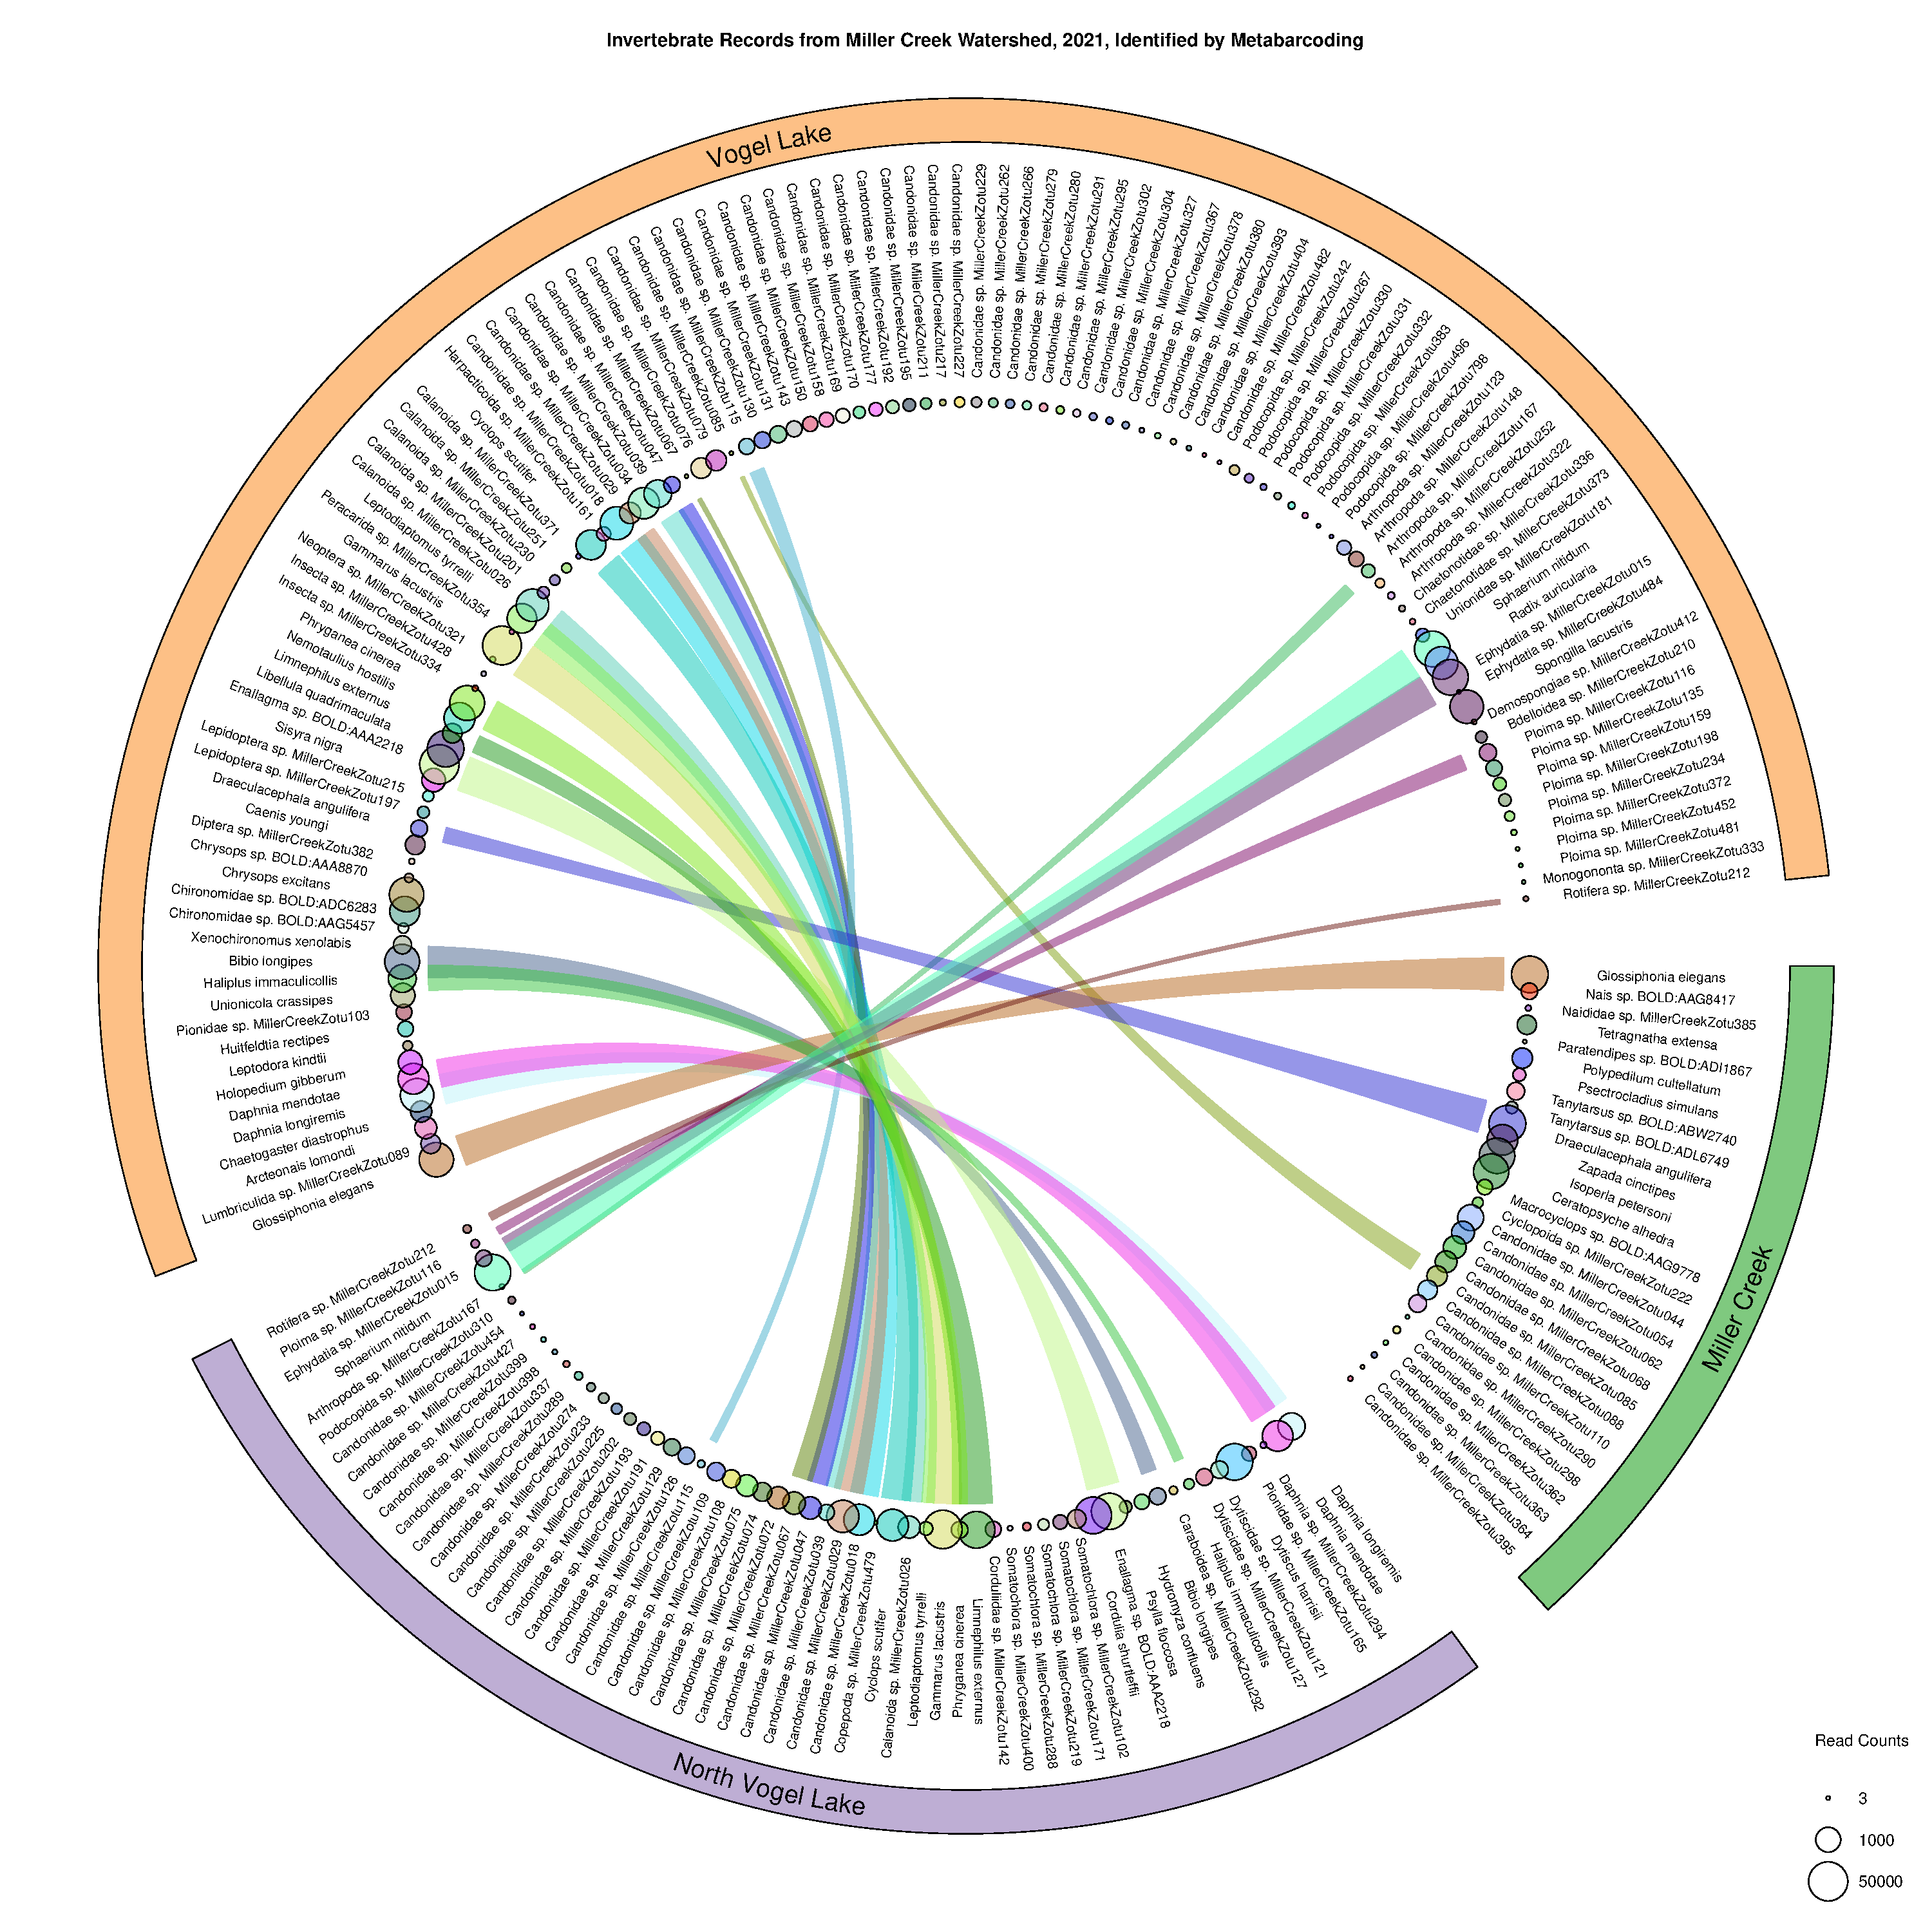
\includegraphics[width=\textwidth]{img/Miller_Creek_network_chord_plot.pdf}
\caption{Chord plot of identifications obtained by metabarcoding from the Miller Creek watershed in 2021. Sizes of circles correspond to numbers of sequence reads observerd.}
\label{midge_map}
\end{center}
\end{figure} 
\begin{multicols}{2}

\subsection{Methodological concerns}

In all except the plankton samples, we generally observed less diversity in the metabarcoding results than we expected. We suspect that this may have been due to subsampling or inadequate homogenization of samples, resulting in some species not being included in \acr{DNA} extractions. In the future, we may homogenize samples using a blender and cleaning between samples using \acr{DIY-DS} as described by \citet{Buchneretal2021} before shipping samples out for metabarcoding.

In future metagenomic analyses we may retain sequences from non-target taxonomic groups as recommended by \citet{Zafeiropoulosetal2021}.

\section{Acknowledgments}

We thank \href{https://www.inaturalist.org/}{iNaturalist.org} people \verb|amr_mn| and \verb|zvkemp| (Zach Kemp) for identifications.

\bibliography{Miller_Creek_inventory}


